\documentclass{cup-pan}
\usepackage[utf8]{inputenc}
\usepackage{blindtext}
\usepackage{xfrac}
\usepackage{graphicx}

\title{The Exponential Curve is Cool as Shit}

\author[1]{Steven Hurwitt}


\affil[1]{M.S. Statistics University of Illinois, Urbana-Champaign, 240 W. 23rd St. Houston, TX. Email: \url{stevenhurwitt@gmail.com}}

%% Corresponding author
\corrauthor{Steven Hurwitt}

%% Abbreviated author list for the running footer
\runningauthor{Steven Hurwitt}

% \addbibresource{refs.bib}
%\texttt{nosupp}

\begin{document}

\maketitle

\begin{abstract}
Appealing properties of the exponential curve (and families) are discussed, along with important real-world examples.
\keywords{statistics, mathematics, finance, exponential trends.}
\end{abstract}



\section{Introduction}
\label{sec:intro}
\paragraph{}
The exponential curve is cool as shit. In this article I will attempt to detail some of the unique features of exponential functions, along with some interesting applications \footnote{for a seemingly random number, it pops up everywhere in nature}. When you're cooking dinner and heating up an oven or a stove, this phenomena has exponential properties with a relation to time \footnote{how easy is it to burn something once the pan starts heating up?}. Of course, these properties also work in reverse. While you're waiting for the food to cool down, it's again undergoing an exponential relationship with respect to both temperature and time \footnote{so it immediately cools down, with the rate slowing with the passing of time, until it reaches an equilibrium. This can be proved by looking at the derivatives - more on this later}.

\paragraph{}
This same logic holds for a variety of phenomena involving exponential curves - for example, in your bank account (or credit card!!) - as well as population growth, and more. My main argument is two-fold, with the first part being essentially that the exponential curve is neat. The second is that understanding it a little further can have real-world implications, with respect to finance, biology, statistics, and (in my opinion) human nature \footnote{my final plea is to not be too intimidated with equations (they can't hurt you)}. If you felt that math was not your strong suite in school, then you are exactly the type of person to whom I'm writing this little article.

\section{History of \textit{e}}
\label{sec:history}
\paragraph{}
Lets start with a little background, in order to fully appreciate the beauty of this little number, \textit{e}. It's more famous cousin is most definitely $ \pi$, although I argue that \textit{e} is much more widespread and interesting than $ \pi$. While $\pi$ is defined as the ratio of a circle's circumference (the length of a circle if it were unfolded) to the circle's diameter (the length across a circle), \textit{e} is little more complicated.

\paragraph{}
The discovery of \textit{e} started with a question: what if an account had one dollar in it and was credited with $100 \%$ interest at the end of the year? What if it was credited more frequently? For the first scenario, the calculation is quite simple, your balance at the end of the year would be two dollars. For the second scenario, we have to do a little math. Let's assume the account is credited with interest once a month (twelve times a year). The future value would then be $$ \$1 \cdot (1 + \sfrac{1}{12} )^{12} = \$ 2.61$$

\paragraph{}
Taking this question a step further, what would happen if we were to \textit{compound} (i.e. dish out) this interest more and more frequently \footnote{still at 100 \%, mind you, everyone in the world would be signing up for this bank account}? Mathematically, this is equivalent to taking the limit of a more general function:
$$\lim_{n \to \infty} (1 + \sfrac{1}{n})^{n} = 2.71828$$

For reasons beyond the scope of this little article, this limit ends up equalling \textit{e}. To add just one more (okay, well two, really) equations to this, the exponential function is defined as: $$y = \textit{e}^{x} \text{, or } y = \exp\{x\}.$$

\paragraph{}
This also leads us to another concept, the logarithm. Specifically we are interested in the natural logarhitm. It is really just the inverse function of \textit{e}.  It is defined as the value $x$, such that $$x = \log ( y )$$ where log here indicates the \textit{natural logarithm}. What this means is for, say, $x = 2$ we can calculate $y = \textit{e}^2 = 7.389.$ Therefore, we would expect $y = \log (7.389) = 2$.

\paragraph{} 
These two concepts (hopefully) seem simple, but give rise to some powerful mathematical concepts (or maybe I'm just a nerd, either way). As an additional note, the above equation details an \textit{exponential increase}, while an exponential decrease would be notated much the same, except with a negative variable, i.e. $$y = \textit{e}^{-x}.$$

\section{Applications}
\label{sec:apps}

\paragraph{}
We now get to the "interesting part" - where does this little equation show up and how exactly is it relevant to us? Thomas Pynchon's novel, \textit{Gravity's Rainbow}, describes the bombing in London as such:

\begin{quote}
For instance, if on average London received one rocket strike per square kilometer per day, the Poisson equation could be used to predict the probability of a random $1 \text{km}^2$ area of London receiving 0, 1, 10 or any other number of rocket strikes. Of relevance to the novel, a necessary assumption of the Poisson distribution is that events are independent: even if a given square kilometer of London has already received 100 rocket strikes today, it is still just as likely to be hit again as any other square kilometer of London.
\end{quote}

The poisson distribution is of course, a member of the \textit{exponential family} in statistics and takes the rate of an event ocurring, $\lambda$, to give the equation: $$f(x| \lambda) = \frac{\lambda^x}{x!} \textit{e}^{-\lambda}.$$

More on exponential families in a bit. To further explain the mathematical notation, $x$ represents the data we are collecting, while $\lambda$ represents a fixed \textit{parameter} of the distribution. It is read as $f(x) \textit{ given } \lambda$, where $\lambda$ is simply the average number of occurrences.

\subsection{Population}
\paragraph{}
From a biological perspective, population growth is an exponential phenomenon. Given an unlimited set of resources \footnote{for something, say, like bacteria}, a population will grow exponentially. This model can be tweaked a little bit into a \textit{logistic} model, which says the growth will level off at the \textit{carrying capacity}. Example figures \ref{fig:pop_growth} are given:

\begin{figure}[h!]
 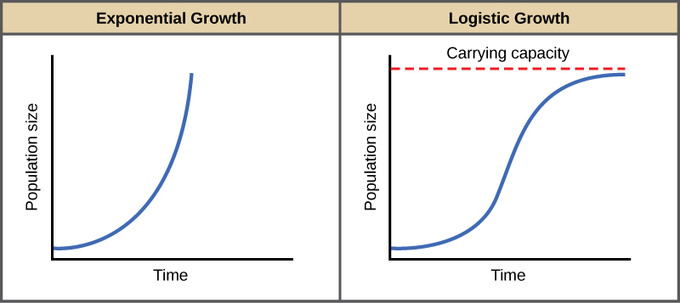
\includegraphics[width=\linewidth]{population_growth.jpeg}

\caption{\textbf{Exponential and logistical population growth}: When resources are unlimited, populations exhibit exponential growth, resulting in a J-shaped curve. When resources are limited, populations exhibit logistic growth. In logistic growth, population expansion decreases as resources become scarce, leveling off when the carrying capacity of the environment is reached, resulting in an S-shaped curve.}
\label{fig:pop_growth}
\end{figure}

\paragraph{} This brings us to a (slightly) more complicated exponential model: $$y = C\textit{e}^{kx}$$
where $C$ is the initial population size and $k$ is the rate of increase. Note that this model is flexible - it can be used in this case of population growth, but it can also be used to represent heating or cooling \footnote{discussed in the intro}, compound interest \footnote{discussed in the history}, along with other natural and man-made phenomena.

\paragraph{Exercise} The following is an exercise for the reader. Collect world population data for the past few hundred (or thousand) years and try to fit an exponential (or logistic) model to the data. Where are we on the population curve? Can we use this to predict when there will be (more) global struggle for resources, etc.? Basically can we use this to predict when the world will end?

\subsection{Technology}
Technology (to me) is a more natural occurrence of exponential phenomena. The most famous of this is definitely \textit{Moore's Law} of  integrated circuits. Essentially, this law says that 

\begin{quote}
...the number of transistors that can be placed on an integrated circuit for the same price will increase exponentially by a factor of 2 every 18 to 24 months. In other words, put simply Moore's Law claims that CPU processing power will double approximately every two years for the price of 1,000 dollars.
\end{quote}

\paragraph{}
Of course this has profound implications for computing that we have seen pretty clearly in the past few decades \footnote{how much have computers improved in your lifetime? in mine I have seen us go from box-looking desktops using dial-up internet to smart phones, laptops, and more - pretty cool. more on this in a future article (hopefully).}. 

\paragraph{}
It's interesting (to me) to look at the progress we have made with computers (such a powerful tool that almost everyone takes for granted). In the early 1900s, computers were rooms of women who would perform calculations such as the \textit{mean squared error} for statistical models. This went on to a giant computer that filled a room, computers that took punch cards for code, personal computers, the internet, laptop computers with GPUs, etc, etc.

\paragraph{}
The following figure \ref{fig:moore} shows the growth of computing techonology throughout the 1900s.

\begin{figure}[h!]
\centering
 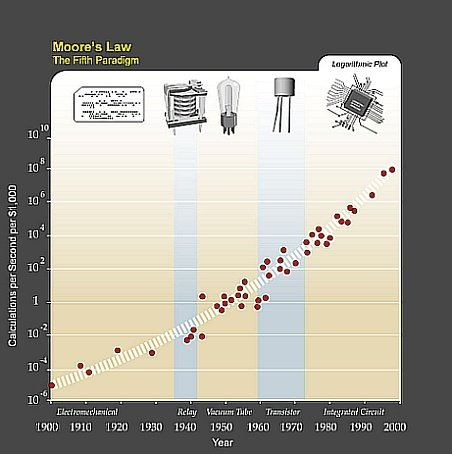
\includegraphics[scale = .5]{moores_law.jpg}

\caption{Moore's law detailing the growth of computers in the 20th century.}
\label{fig:moore}
\end{figure}

\subsection{Finance}
\paragraph{}
Exponential relationships are also pretty big in the world of finance. For example, let's look at different calculations relating to the closing stock price of Google (GOOGL).

\begin{table}[ht!]
\caption{Google Stock Closing Price. Source: \url{https://finance.yahoo.com/quote/GOOG/history?p=GOOG}}
\label{tab:goog}
\centering
\begin{tabular}{l l l l r}
\headrow \thead{Date} & \thead{Close} \\
Mar 26, 2020     & \$ 1,111.80   \\
Mar 25, 2020     & \$ 1126.47 \\
Mar 24, 2020     & \$ 1103.77  \\
Mar 23, 2020     & \$ 1061.32 \\
Mar 20, 2020     & \$ 1135.72 \\

\end{tabular}

\end{table}

\paragraph{}
When looking at stock prices, there a few metrics we can use to evaluate it. These include the \textit{simple moving average (SMA)}, \textit{weighted moving average (WMA)} and \textit{exponentially-weighted moving average (EMA).} We can perform these calculations using the following formulas:

$$\text{SMA} = \frac{P_1 + P_2 + ... + P_n}{n}$$

$$\text{WMA} = P_n \cdot \text{weight factor} + P_{n-1} \cdot (\text{weight factor} - 1)$$

$$\text{EMA} = (P_n - \text{previous EMA}) \cdot \frac{2}{n + 1} + \text{previous EMA}$$

\paragraph{}
These calculations help signal traders how well (or poorly) a given stock is doing. They can be calculated simply (with a calculator), with formulas (Excel), or through code (Python, etc).

\paragraph{} There are also examples of exponential relationships in calculating the future value of income with a certain interest rate over time \footnote{compound interest was the example used earlier.}.

\paragraph{Exercise} Calculate these moving averages for the Google closing price. Use a weight of 50 \% (5/10), so the previous weight would be 40 \% (4/10) etc, for these five day closing prices. You could also collect more data and calculate them with a larger window.


\subsection{Statistics}
\paragraph{} The exponential curve has a multitude of applications in statistics. Most of the probability distributions you learn about in an intro to probability are members of \textit{exponential families} \footnote{mathematical details to come}. Some examples include the bernoulli, binomial, poisson \footnote{described earlier}, negative binomial, beta, gamma, exponential, pareto and of course, the normal distributions.

\paragraph{} The normal distribution \footnote{described by one of my professor who said the Central Limit Theorem is basically the Statisticians' Employment Theorem} is a bell-shaped curve with a very complicated-looking equation. This distribution generally describes averages, for example, a random variable such as the height of women, may not be normally distributed, but the average height of women will follow a normal distribution \footnote{provided the sample size is sufficiently large, say 30 or more}.

\paragraph{} The equation assumes a given mean, $\mu$, and standard deviation, $\sigma$:
$$f(x | \mu, \sigma) = \frac{1}{\sqrt{2 \pi \sigma^2}} \textit{e}^{-(x - \mu)^2 / 2 \sigma^2}$$

An example of the curve for population IQ scores where $\mu = 100$ and $\sigma = 15$ is as follows in figure \ref{fig:norm}

\begin{figure}[h!]
\centering
 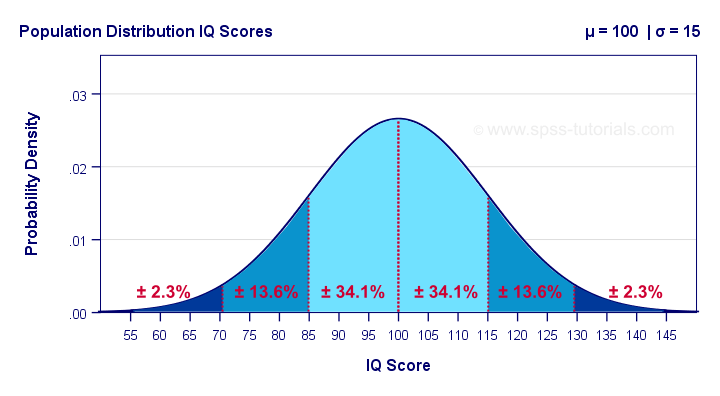
\includegraphics[scale = .4]{norm_dist.png}

\caption{Normal curve showing the percent distribution across a variety of population IQ scores.}
\label{fig:norm}
\end{figure}

\subsection{Calculus and Differential Equations}

\paragraph{}
$y = \textit{e}^x$ also has some appealing properties from a calculus perspective. The \textit{derivative}, which represents the instantaneous rate of change of a function, of this function is $y = \textit{e}^x.$ Using the \textit{chain rule}, the derivative of $$y = C\textit{e}^{kx}$$ would be $$\frac{dy}{dx} = y' = k \cdot C \textit{e}^{kx}.$$

\paragraph{}
This also has implications for the integral of $\textit{e}^x$, which is again the same function. Again using the function $$y =A\textit{e}^{kx},$$ the antiderivative will be $$\int f(x) = F(x) = \frac{A}{k} \textit{e}^{kx} + C.$$

\paragraph{}
It will also be helpful to talk about the natural log in relation to integrals and derivatives. The natural log is important. We will talk later about log-linear models. Roughly speaking, if two variables $x$ and $y$ have an exponential relationship, taking the (natural) log of one of the variables might transform the relationship into a \textit{linear relationship}.

\paragraph{} The derivative of $log(x)$ is defined as :
$$y = log(x)$$ 
$$ y' = \frac{1}{x}.$$

This tells us that 
$$ \int \frac{dx}{x} = \int \frac{1}{x} dx = log(x).$$

This fact is useful in \textit{differential equations} where we generally have a problem where the rate of change of some variable is proportional to the variable itself. For example, in a population, if $Y$ is the number of individuals and $r$ is the birth rate, we would say that the rate of change of individuals over time (not accounting for deaths) is expressed as:

$$ \frac{dY}{dt} = rY.$$

This is a \textit{separable differential equation}. In this case, we can get all the Y variables on one side and see:

$$ \frac{dY/dt}{Y} = r.$$
Integrating both sides,
$$\int \frac{dY/dt}{Y} dt = \int r dt$$
$$ \Rightarrow log(Y) = rt + C$$
This is the \textit{log-linear model} mentioned just a second ago. The log of y has a linear relationship with respect to time. Exponentiating both sides, we then see:
$$ \Rightarrow Y = exp\{rt + C \}$$
This can be simplified algebraically, until we end with a (hopefully) familiar equation:
 $$\Rightarrow Y = \textit{e}^{rt} \textit{e}^C$$
$$ \Rightarrow Y = C \textit{e}^{rt}.$$

Of course, this is the general exponential model introduced in the population section.

\section{Conclusions}
\paragraph{}
In this article, we have seen numerous applications of the \textit{exponential curve} and \textit{exponential model}. We saw how it relates to population growth, finances, statistical models and technology. This little number can explain a variety of natural phenomena, as well as those created by humans, such as money and technology.

\paragraph{}
 In my mind, it's cool when there's a relationship between nature and technology. To me, nature and natural laws are pre-existing and governed by physical laws. Discovering these is sort of like discovering the language of gods and how they think and design things. In this way, the man-made phenomena are also interesting. Advances in computing are spawning different ways of human functioning \footnote{both good and bad, I could go on and on about the pros and cons of tech...}

\section{Mathematical Background}
\label{sec:math}

\paragraph{}
After delving into some mathematical details about differential equations, this section shall be for the more mathematically-inclined curious reader. The main discussion is of exponentially families and neat properties of them.

\paragraph{} An exponential family of distributions is described in terms of the data, $x$ and parameters, $\theta$. In most cases $\theta$ represents parameters such as the true mean or standard deviation. In past examples $\lambda$ and the mean $\mu$ and standard deviation $\sigma$ were our parameters of interest.

\paragraph{} Mathematically, an exponential family is one defined as:

$$f(x|\theta) = exp\big\{ \eta(\theta) \cdot t(x) - B(\theta) \big\} h(x) $$

where it can be shown that $t(x)$ is a \textit{sufficient statistic}. These are generally things such as the sum of x or the average, meaning that this quantity can sufficiently describe the data.

\paragraph{}
Using the poisson distribution from earlier, if we define the function in terms of $\theta$,

$$\frac{\theta^x}{x!} \textit{e}^{-\theta} = exp \big\{ (log \theta) x - \theta \big\} \frac{1}{x!}$$ 

so we see that: 

$$\eta(\theta) = log \theta, t(x) = x, B(\theta) = \theta, \text{ and } h(x) = \frac{1}{x!}.$$

This tells us that $x$ is a sufficient statistic for the Poisson distribution. This can similarly be proved for all of the other "standard" statistical distributions, using a little algebra.

\vspace{10mm}

\section{References}

\begin{enumerate}
\item \url{https://www.ugrad.math.ubc.ca/coursedoc/math100/notes/diffeqs/cool.html}
\item \url{https://en.wikipedia.org/wiki/E_(mathematical_constant)}
\item \url{https://gravitys-rainbow.pynchonwiki.com/wiki/index.php?title=Pages_53-60}
\item \url{https://courses.lumenlearning.com/boundless-biology/chapter/environmental-limits-to-population-growth/}
\item \url{http://www.singularitysymposium.com/moores-law.html}
\item \url{https://www.thebalance.com/simple-exponential-and-weighted-moving-averages-1031196}
\item \url{https://www.spss-tutorials.com/normal-distribution/}
\item \url{https://www2.stat.duke.edu/courses/Spring11/sta114/lec/expofam.pdf}
\end{enumerate}

\end{document}